\documentclass[11pt]{scrartcl}

% ---------- Packages ----------
\usepackage[margin=1in]{geometry}
\usepackage{mathpazo}
\usepackage{amsmath,amssymb,amsthm}
\usepackage{tikz}
\usetikzlibrary{arrows.meta,positioning}
\usepackage[most]{tcolorbox}
\usepackage{xcolor}
\usepackage{hyperref}

% ---------- Colors ----------
\definecolor{accentblue}{RGB}{44,95,138}
\definecolor{boxfill}{RGB}{240,245,250}
\definecolor{boxborder}{RGB}{180,200,220}
\definecolor{highlightred}{RGB}{200,50,50}

% ---------- Theorem environments ----------
\newtcolorbox{thmbox}[1]{
  colback=boxfill, colframe=boxborder,
  boxrule=0.6pt, arc=2pt, left=6pt, right=6pt, top=4pt, bottom=4pt,
  fonttitle=\bfseries\color{accentblue}, title=#1
}
\theoremstyle{plain}
\newtheorem{theorem}{Theorem}
\theoremstyle{remark}
\newtheorem*{remark}{Remark}

\hypersetup{colorlinks=true, linkcolor=accentblue, urlcolor=accentblue}

\title{\color{accentblue}Eulerian Graphs and Digraphs}
\author{}
\date{}

\begin{document}
\maketitle

% =========================================================
\begin{thmbox}{Lemma 1}
If $G$ is a graph in which the degree of each vertex is at least two, then $G$ contains a cycle.
\end{thmbox}

\begin{proof}[Proof 1]
If $G$ is a simple graph, let $v_0$ be any vertex of $G$. We construct a walk $v_0 \to v_1 \to \cdots$ inductively, by choosing $v_{i+1}$ to be any vertex adjacent to $v_i$; the existence of this vertex is guaranteed by our hypothesis. Since $G$ has only finitely many vertices, we must eventually choose a vertex that has been chosen before, and the walk between its two occurrences is a cycle.
\end{proof}

\begin{proof}[Proof 2 (sketch)]
$G$ is not a tree.
\end{proof}

\begin{remark}
The notes leave this alternative argument as a brief hint, without further elaboration.
\end{remark}

% =========================================================
\begin{thmbox}{{Theorem 2 (Euler, 1736)}}
A connected graph is Eulerian $\iff$ the degree of each vertex is even.
\end{thmbox}

\begin{proof}
($\Rightarrow$) Suppose that $P$ is an Eulerian trail in $G$. Whenever $P$ passes through a vertex, there is a contribution of $2$ towards the degree of that vertex ($\to v \to$); since each edge occurs exactly once in $P$, each vertex must have even degree.

\medskip
\noindent ($\Leftarrow$) The proof is by induction on the number of edges of $G$. Suppose that the degree of each vertex is even. Since $G$ is connected, each vertex has degree at least $2$, and so by Lemma 1, $G$ contains a cycle $C$. If $C$ contains every edge of $G$, the proof is complete. If not, we remove from $G$ the edges of $C$, to form a possibly disconnected graph $H$ with fewer edges than $G$, in which each vertex still has even degree. By induction, each component of $H$ has an Eulerian trail. Since each component of $H$ has at least one vertex in common with $C$, by connectedness we obtain the required Eulerian trail of $G$ by following the edges of $C$ until a non-isolated vertex of $H$ is reached, tracing the Eulerian trail of the component of $H$ that contains that vertex, and then continuing along the edges of $C$; the whole process terminates when we reach the initial vertex.
\end{proof}

\medskip
\noindent This proof can easily be modified to prove the following results.

% =========================================================
\begin{thmbox}{Corollary 1}
A connected graph is Eulerian $\iff$ it can be split (as a set of edges) into disjoint cycles.
\end{thmbox}

\begin{remark}
No separate proof was given in the original notes; the modification of the proof of Theorem 2 is indicated but not written out.
\end{remark}

% =========================================================
\begin{thmbox}{Corollary 2}
A connected graph is semi-Eulerian $\iff$ it has exactly two vertices of odd degree.
\end{thmbox}

\begin{proof}
($\Rightarrow$) Assume we have a trail $T$ from $u$ to $v$. If we add an edge between $v$ and $u$, we obtain an Eulerian graph (all vertices have even degree); if we remove that edge, only $u$ and $v$ have odd degree.

\medskip
\noindent ($\Leftarrow$) We add an edge between these two vertices; then all vertices have even degree, so it is an Eulerian graph.
\end{proof}

% =========================================================
\begin{thmbox}{{Theorem 3 (Fleury's Algorithm)}}
Let $G$ be an Eulerian graph. Then the following construction is always possible and produces an Eulerian trail of $G$. Start at any vertex $u$ and traverse the edges in any way, subject to this rule:
\begin{enumerate}
  \item Erase each edge as it is traversed, and if any isolated vertex results, erase it too.
  \item At each stage, use a bridge only if there exists no alternative.
\end{enumerate}
\end{thmbox}

\begin{proof}
We first show that the construction can be carried out at each stage. Suppose that we have just reached a vertex $v$. If $v \neq u$, then the subgraph $H$ that remains is connected and contains only two vertices of odd degree, $u$ and $v$. To show that the construction can be carried out, we must show that the removal of the next edge doesn't disconnect $H$, or equivalently, that $v$ is incident with at most one bridge.

But if this is not the case, then there exists a bridge $vw$ such that the component $K$ of $H - vw$ containing $w$ does not contain $u$. Since the vertex $w$ has odd degree in $K$, some other vertex of $K$ must also have odd degree, giving the required contradiction.

\begin{center}
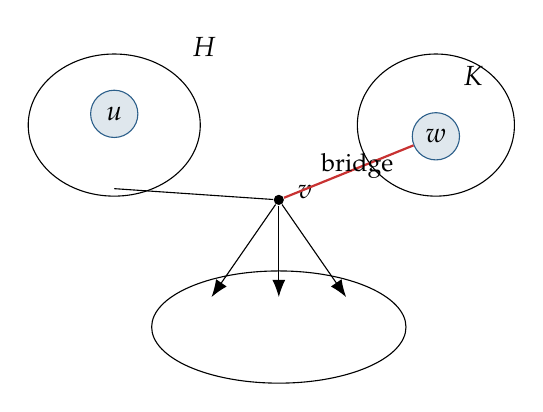
\begin{tikzpicture}[scale=0.95]
  \node[circle,fill=black,inner sep=1.3pt] (v) at (0,0) {};
  \node[draw=none,fill=none] at (0.35,0.1) {$v$};

  \draw (-2.2,1.0) ellipse (1.15 and 0.95);
  \node[circle,draw=accentblue,fill=accentblue!15,minimum size=6mm,inner sep=0pt] (u) at (-2.2,1.15) {$u$};
  \node[draw=none,fill=none] at (-1.0,2.05) {$H$};
  \draw (v) -- (-2.2,0.15);

  \draw (2.1,1.0) ellipse (1.05 and 0.95);
  \node[draw=none,fill=none] at (2.6,1.65) {$K$};
  \node[circle,draw=accentblue,fill=accentblue!15,minimum size=6mm,inner sep=0pt] (w) at (2.1,0.85) {$w$};
  \draw[highlightred, thick] (v) -- (w);
  \node[draw=none,fill=none] at (1.05,0.45) {\small bridge};

  \draw (0,-1.7) ellipse (1.7 and 0.75);
  \foreach \x in {-0.9,0,0.9}{
    \draw[-{Latex[length=2.2mm]}] (v) -- (\x,-1.3);
  }
\end{tikzpicture}
\end{center}

If $v = u$, the proof is almost identical, as long as there are still edges incident with $u$.

It remains only to show that this construction always yields a complete Eulerian trail. But this is clear, since there are no edges of $G$ remaining untraversed when the last edge incident to $u$ is used: otherwise, the removal of some smaller edge adjacent to one of these edges would have disconnected the graph, contradicting rule 2.
\end{proof}

% =========================================================
\begin{thmbox}{Theorem 4}
A strongly connected digraph $D$ is Eulerian $\iff$ for each vertex $v$ of $D$, $\operatorname{outdeg}(v) = \operatorname{indeg}(v)$.
\end{thmbox}

\begin{proof}
($\Rightarrow$) Suppose $D$ has an Eulerian trail. Each time the trail enters a vertex $v$, it uses one incoming arc; each time it leaves $v$, it uses one outgoing arc. Since every arc appears exactly once in the trail, $\operatorname{outdeg}(v) = \operatorname{indeg}(v)$.

\medskip
\noindent ($\Leftarrow$) We proceed by induction on the number of arcs; the result is trivial for no arcs. Assume the theorem holds for all connected digraphs with fewer arcs than $D$. Since $D$ is connected and every vertex satisfies $\operatorname{outdeg}(v) = \operatorname{indeg}(v)$, every vertex has at least one outgoing arc. Starting from any vertex and repeatedly following outgoing arcs, because the graph is finite, we must eventually repeat a vertex. Hence $D$ contains a directed cycle $C$.

If $C$ contains all arcs, the proof is complete. Otherwise, we remove the arcs of $C$ from $D$, obtaining a digraph, possibly disconnected, $H$. Each component of $H$ has fewer arcs than $D$, so it has an Eulerian trail. Moreover, since $D$ is connected, every component of $H$ shares at least one vertex with the cycle $C$.

We now construct an Eulerian trail of $D$: start traversing the directed cycle $C$; when a vertex is reached that belongs to $H$ with unused arcs, traverse the Eulerian trail of that component of $H$, then continue along $C$; the resulting trail is a directed Eulerian trail of $D$.
\end{proof}

\end{document}
